% acex13.tex/06/24/2013\documentclass[mathserif]{beamer}%
\documentclass{beamer}
\usepackage{amsxtra,amssymb,amsthm,amsmath,latexsym}
\usepackage{multicol}
\usepackage{beamerthemesplit}
%\usetheme{Darmstadt}
\numberwithin{equation}{section}
\newtheorem{thm}{Theorem}[]
\newcommand{\EN}{\mathcal{N}}
\newcommand{\na}{\nabla}
\newcommand{\R}{{\mathbb R}}
\newcommand{\ra}{\rightarrow}
\newcommand{\ue}{\infty}
\newcommand{\nc}{\newcommand}
\newcommand{\RRR}{\mathbb{R}^3}
\newcommand{\ol}{\overline}
\newcommand{\thmref}[1]{Theorem~\ref{#1}}
\newcommand{\lemref}[1]{Lemma~\ref{#1}}
\newcommand{\xy}{\boldsymbol{x}}
\newcommand{\uv}{\boldsymbol{u}}
\newcommand{\conv}{\circledast}
\newcommand{\llangle}{\left\langle}
\newcommand{\rrangle}{\right\rangle}
\def\bee{\begin{equation*}}
\def\eee{\end{equation*}}
\def\be{\begin{equation}}
\def\ee{\end{equation}}
\nc{\Ba}{\Big(} \nc{\Bz}{\Big)} \nc{\pa}{\partial} \nc{\ti}{\times}
\nc{\n}{|} \nc{\al}{\alpha} \nc{\da}{\delta} \nc{\bs}{\backslash}
\nc{\ka}{\kappa} \nc{\Da}{\Delta} \nc{\si}{\sigma} \nc{\f}{\big(}
\nc{\g}{\big)}
%\nc{\n}{|}
\nc{\om}{\omega}
\begin{document}
%%%% Test - Einsatz  Kapitel 5 -
\part{ }
%XXXXXXXXXXXXXXXXXXXXXXXXXXXXXXXXXXXXXXXXXXXXXXXXXXXX
\title[CIRL Discusson]{9/6/19 Discussion}
\institute{}
\date{}
\frame{\titlepage}
\section{Using GPU for model-based methods}
\frame{
Problem with model-based methods:
\begin{itemize}
\item[1.] large memory requirement because of caching the up-sampled data $g^{\text{HR}}$, $i_m, j_m$ and FFT/IFFT computation, for example, to compute $g(\xy,z) = \sum_{m = 1}^{N_m} [o(\xy,z)j_m(\xy)]\conv[h(\xy,z)i_m(z)]$ in the forward model.
\item[2.] low performance due to the FFT/IFFT computation.
\end{itemize}
Improvement ideas using GPU: 3x faster performance and 4x less memory requirement when
\begin{itemize}
\item[1.] computing the up-sampled data, $i_m, j_m$ on the fly using GPU.
\item[2.] doing the FFT/IFFT on GPU.
\end{itemize}
Problem still: doing FFT/IFFT on GPU requires large GPU memory. Maybe one only needs to use GPU to compute $i_m, j_m$ and to up-sample the LR data (note that up-sampling the LR data requires FFT/IFFT).
}

\section{3D star-like object}
\frame{
On $xy, xz$ planes
\begin{figure}[H]
  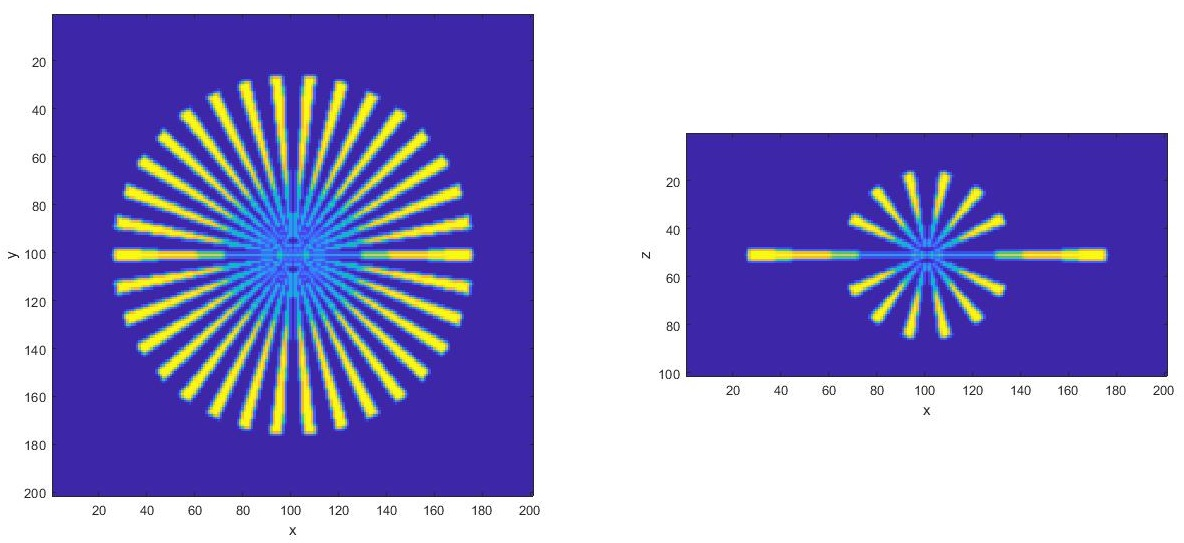
\includegraphics[width=\linewidth]{pics/3DStarLikeXYXZ}
\end{figure}
}
\frame{
\begin{figure}[H]
  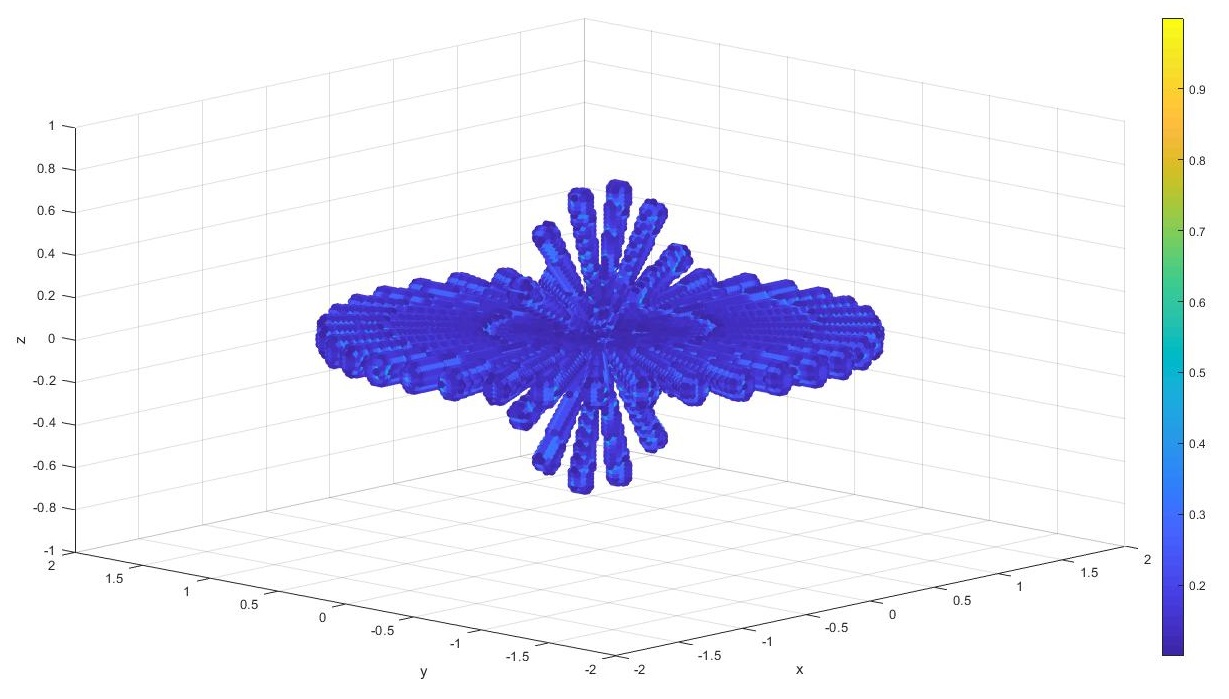
\includegraphics[width=\linewidth]{pics/3DStarLike}
\end{figure}
}

\section{Next tasks}
\frame{
\begin{itemize}
\item[1.] FairSIM data: try model-based methods with FairSIM data, investigate parameters in FairSIM.
\item[2.] Run simulation with data reduction and model-based methods on current multi-object, for both 3W and Tunable.
\item[3.] Formulate 3D star-like object and run simulation on 3D star-like object.
\end{itemize}
}

%% #
%\frame[shrink=30]{\frametitle{Test}
%Test
%}

\end{document}
